\chapter{DESAIN DAN IMPLEMENTASI}
\vspace{1ex}

\section*{}
	Penelitian ini dilaksanakan sesuai dengan desain sistem berikut dengan implementasinya. Desain sistem merupakan konsep dari pembuatan dan perancangan infrastruktur kemudian diwujudkan dalam bentuk blok-blok alur yang harus dikerjakan. Pada bagian implementasi merupakan pelaksanaan teknis untuk setiap blok pada desain sistem.
\vspace{1ex}

\section{Desain Sistem}
\vspace{1ex}
Penelitian ini merupakan penerapan dari bidang studi \textit{Mobile
Programming, Internet of Things, Signal processing}, dan Basis data. Penitian ini memiliki tujuan untuk
mengakuisisi data sinyal jantung menggunakan sensor AD8232 dan menyimpan data sinyal tersebut kedalam databse untuk dapat ditampilkan pada aplikasi smartphone pasien dan dokter sehingga dokter dapat memantau kondisi pasien serta memberikan diagnosa, dokter dan pasien juga dapat berkonsultasi melalui fitur chat yang ada pada aplikasi android. Berikut merupakan desain sistem dari penelitian ini.

\vspace{1ex}

\begin{figure}[H] \centering
	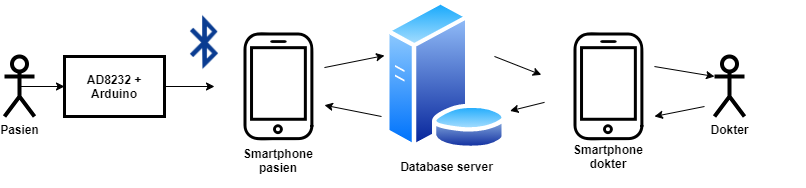
\includegraphics[width=0.9\textwidth]{img/arsitektur.png}
	
	(a)
	
	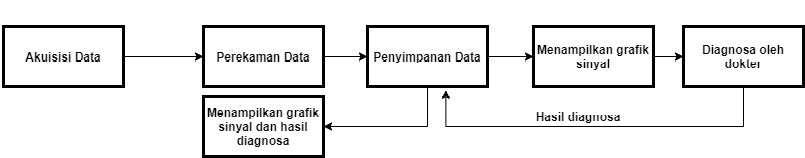
\includegraphics[width=0.9\textwidth]{img/blockdiagram.png}
	
	(b)
	
	\caption{Arsitektur (a) dan Blok Diagram (b) Alur Kerja Sistem}
	\label{fig:3.1}
\end{figure}
\vspace{1ex}

Gambar \ref{fig:3.1} merupakan arsitektur dan
blok diagram alur kerja sistem. Aplikasi android menjadi dapat
mengambil data sinyal jantung pasien yang telah dideteksi
oleh sensor AD8232 melalui modul bluetooth HC-05. Aplikasi
dapat mengirimkan data sinyal jantung pasien kepada dokter
spesialis serta terdapat fitur chatting agar pasien dapat berkonsultasi dengan dokter.
Penelitian ini memiliki bagian tahapan-tahapan yaitu:
\begin{enumerate}
	\vspace{-2mm}
	\item Akuisisi data menggunakan sensor AD8232,
	\vspace{-2mm}
	\item Pengiriman data ECG menuju aplikasi melalui bluetooth HC-05,
	\vspace{-2mm}
	\item Menyimpan data ECG kedalam database,
	\vspace{-2mm}
	\item Menampilkan grafik ECG pada aplikasi android,
	\vspace{-2mm}
	\item Menambahkan fitur chat pada aplikasi android,
	\vspace{-2mm}
	\item Pengujian sistem secara keseluruhan.
\end{enumerate}
\vspace{1ex}

\section{Desain Perangkat}
\vspace{1ex}

Pada penelitian ini menggunakan 3 buah komponen yaitu Arduino Nano, modul bluetooth HC-05, dan sensor AD8232. Rangkaian ketiga komponen tersebut ditunjukkan oleh gambar berikut.
\begin{figure}[H] \centering
	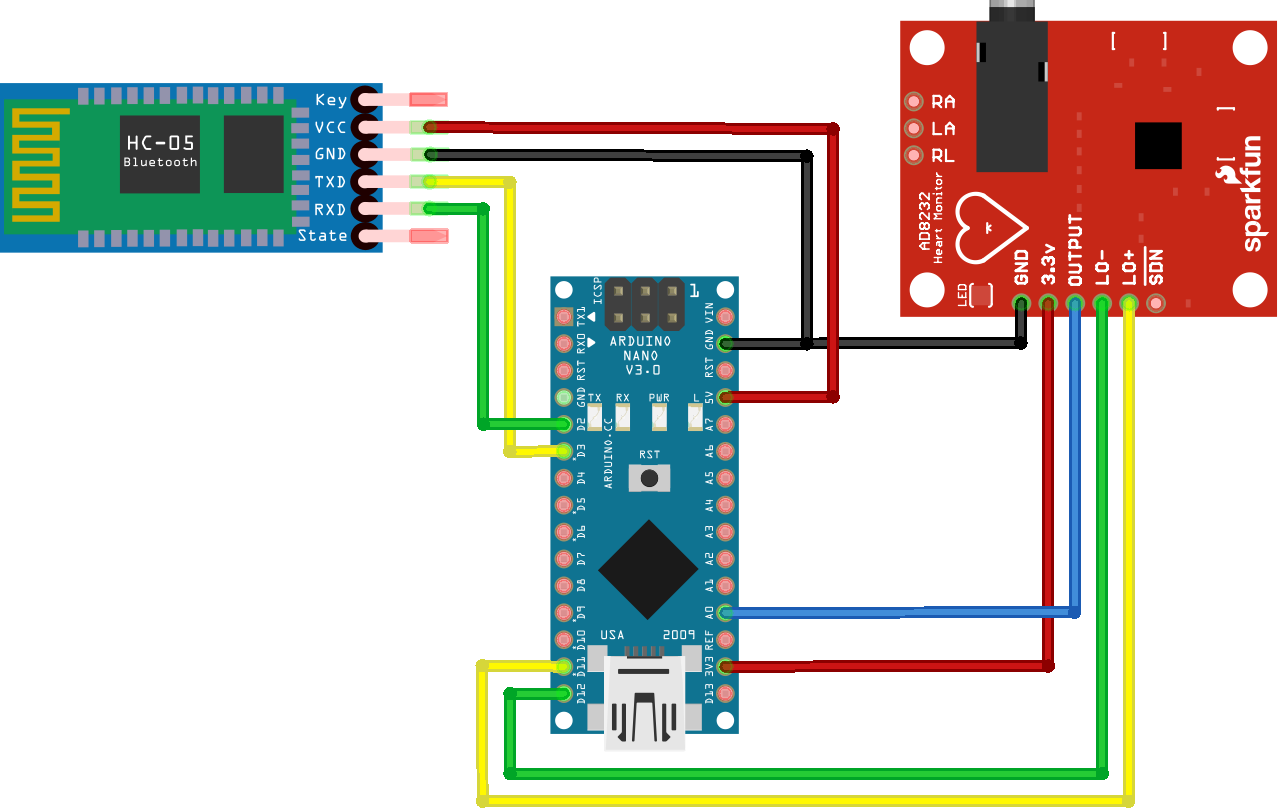
\includegraphics[width=0.9\textwidth]{img/desainperangkat.png}
	\caption{Desain Perangkat ECG}
	\label{fig:3.2.0}
\end{figure}
\vspace{1ex}

Berdasarkan gambar \ref{fig:3.2.0} dapat dilihat sensor AD8232 ada pada posisi paling kanan yang memiliki board berwarna merah. Port AD82332 yang dihubungkan ke Arduino Nano adalah ground, VCC 3.3 Volt, output, LO+, dan LO-. Kemudian pada modul bluetooth HC-05 terdapat 4 port yang dihubungkan pada Arduino Nano yaitu RXD, TXD, GND, dan VCC sebesar antata 3.6 Volt sampai dengan 6 Volt. 
\section{Desain UI Aplikasi}
\vspace{1ex}
Aplikasi android memiliki 2 desain yaitu untuk dokter dan
pasien. Desain UI aplikasi untuk pasien memiliki fitur tambahan. Pada aplikasi pasien memiliki fitur untuk merekam sinyal
ECG sedangkan pada aplikasi dokter tidak disediakan fitur tersebut. Desain aplikasi dokter
ditunjukkan pada Gambar \ref{fig:3.2}.  

\begin{figure}[H] \centering
	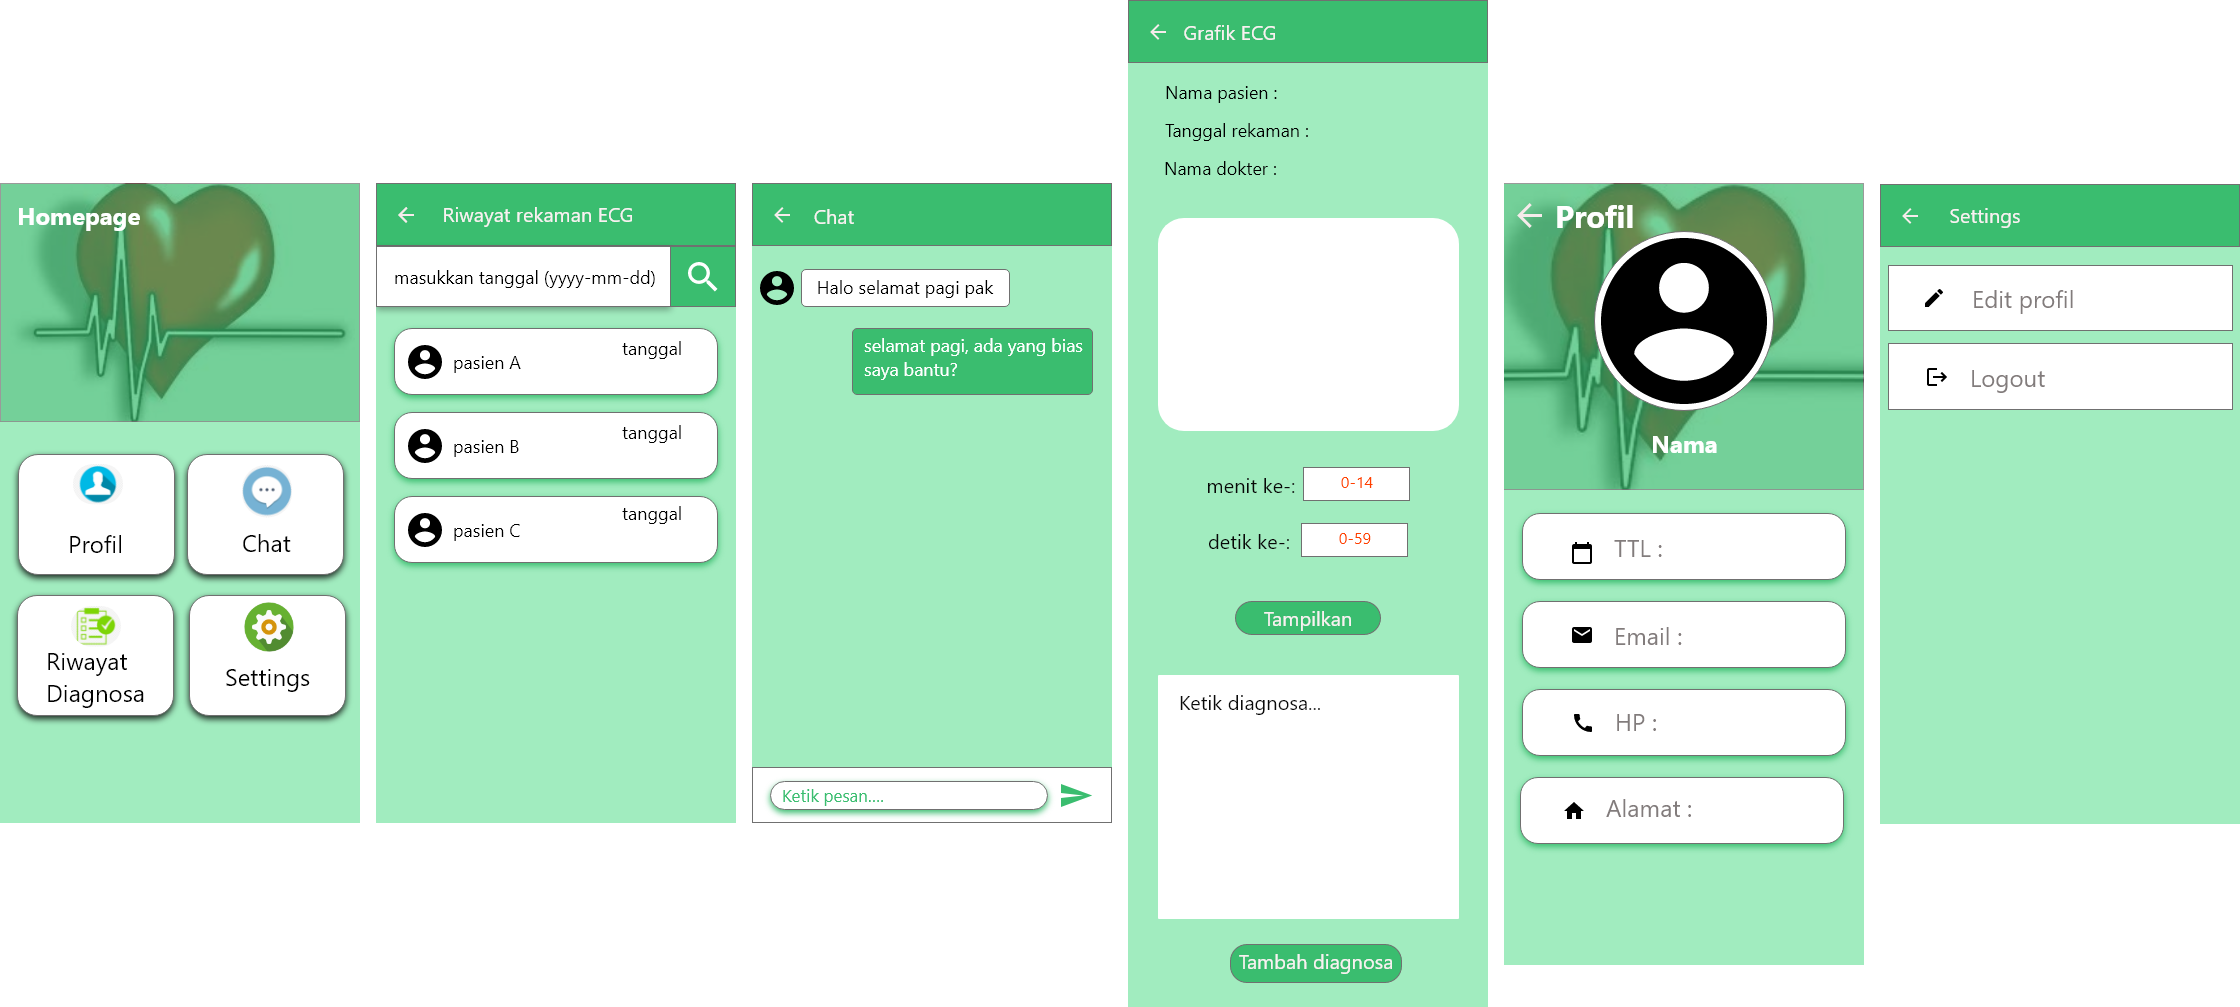
\includegraphics[width=1\textwidth]{img/dokterUI.png}
	\caption{Desain UI pada aplikasi dokter.}
	\label{fig:3.2}
\end{figure}
\vspace{1ex}

Dapat diketahui dari desai UI dokter tersebut terdapat 6 screen, yaitu:
\begin{enumerate}
	\vspace{0mm}
	\item Homepage screen, yang mana merupakan halaman utaman pada aplikasi. Pada Homepage screen dokter tersedia empat buah menu yaitu Profil untuk berpindah ke halaman profil, Chat untuk berpindah ke halaman chat, Riwayat Diagnosa untuk berpindah halaman menuju riwayat diagnosa, dan Settings untuk berpindah ke halaman settings,
	\vspace{0mm}
	\item Riwayat rekaman ECG screen, yang mana merupakan halaman penelusuran yang dapat mencari riwayat ECG pasien pada waktu yang telah diinputkan. Pada screen ini terdapat field untuk menginputkan waktu rekaman dan tombol search untuk mulai mencari. Riwayat rekaman akan ditampilkan dalam bentuk list,
	\vspace{0mm}
	\item Chat screen, yang mana merupakan halaman untuk melakukan komunikasi dengan pasien melalui sebuah pesan,
	\vspace{0mm}
	\item Grafik ECG screen, yang mana merupakan halaman yang dapat menampilkan grafik data ECG hasil rekaman pasien. Pada halaman ini terdapat fitur untuk menampilkan grafik ECG pada waktu tertentu sesuai menit dan detik yang telah diinputkan. Pada halaman ini juga terdapat form isian yang merupakan tempat dokter menambahkan diagnosa untuk pasien,
	\vspace{0mm}
	\item Profil screen, yang mana merupakan halaman yang berisi tentang informasi pengguna. Informasi tersebut antara lain adalah foto, nama lengkap, tanggal lahir, email, nomor telepon, dan alamat,
	\vspace{0mm}
	\item Settings screen, yang mana merupakan halaman yang berisi menu untuk mengubah informasi pada halaman profil dan juga terdapat menu \textit{logout} untuk keluar dari aplikasi.
\end{enumerate}

\clearpage
Berikutnya adalah desain UI untuk pasien ditunjukkan pada Gambar \ref{fig:3.3}.
\begin{figure}[H] \centering
	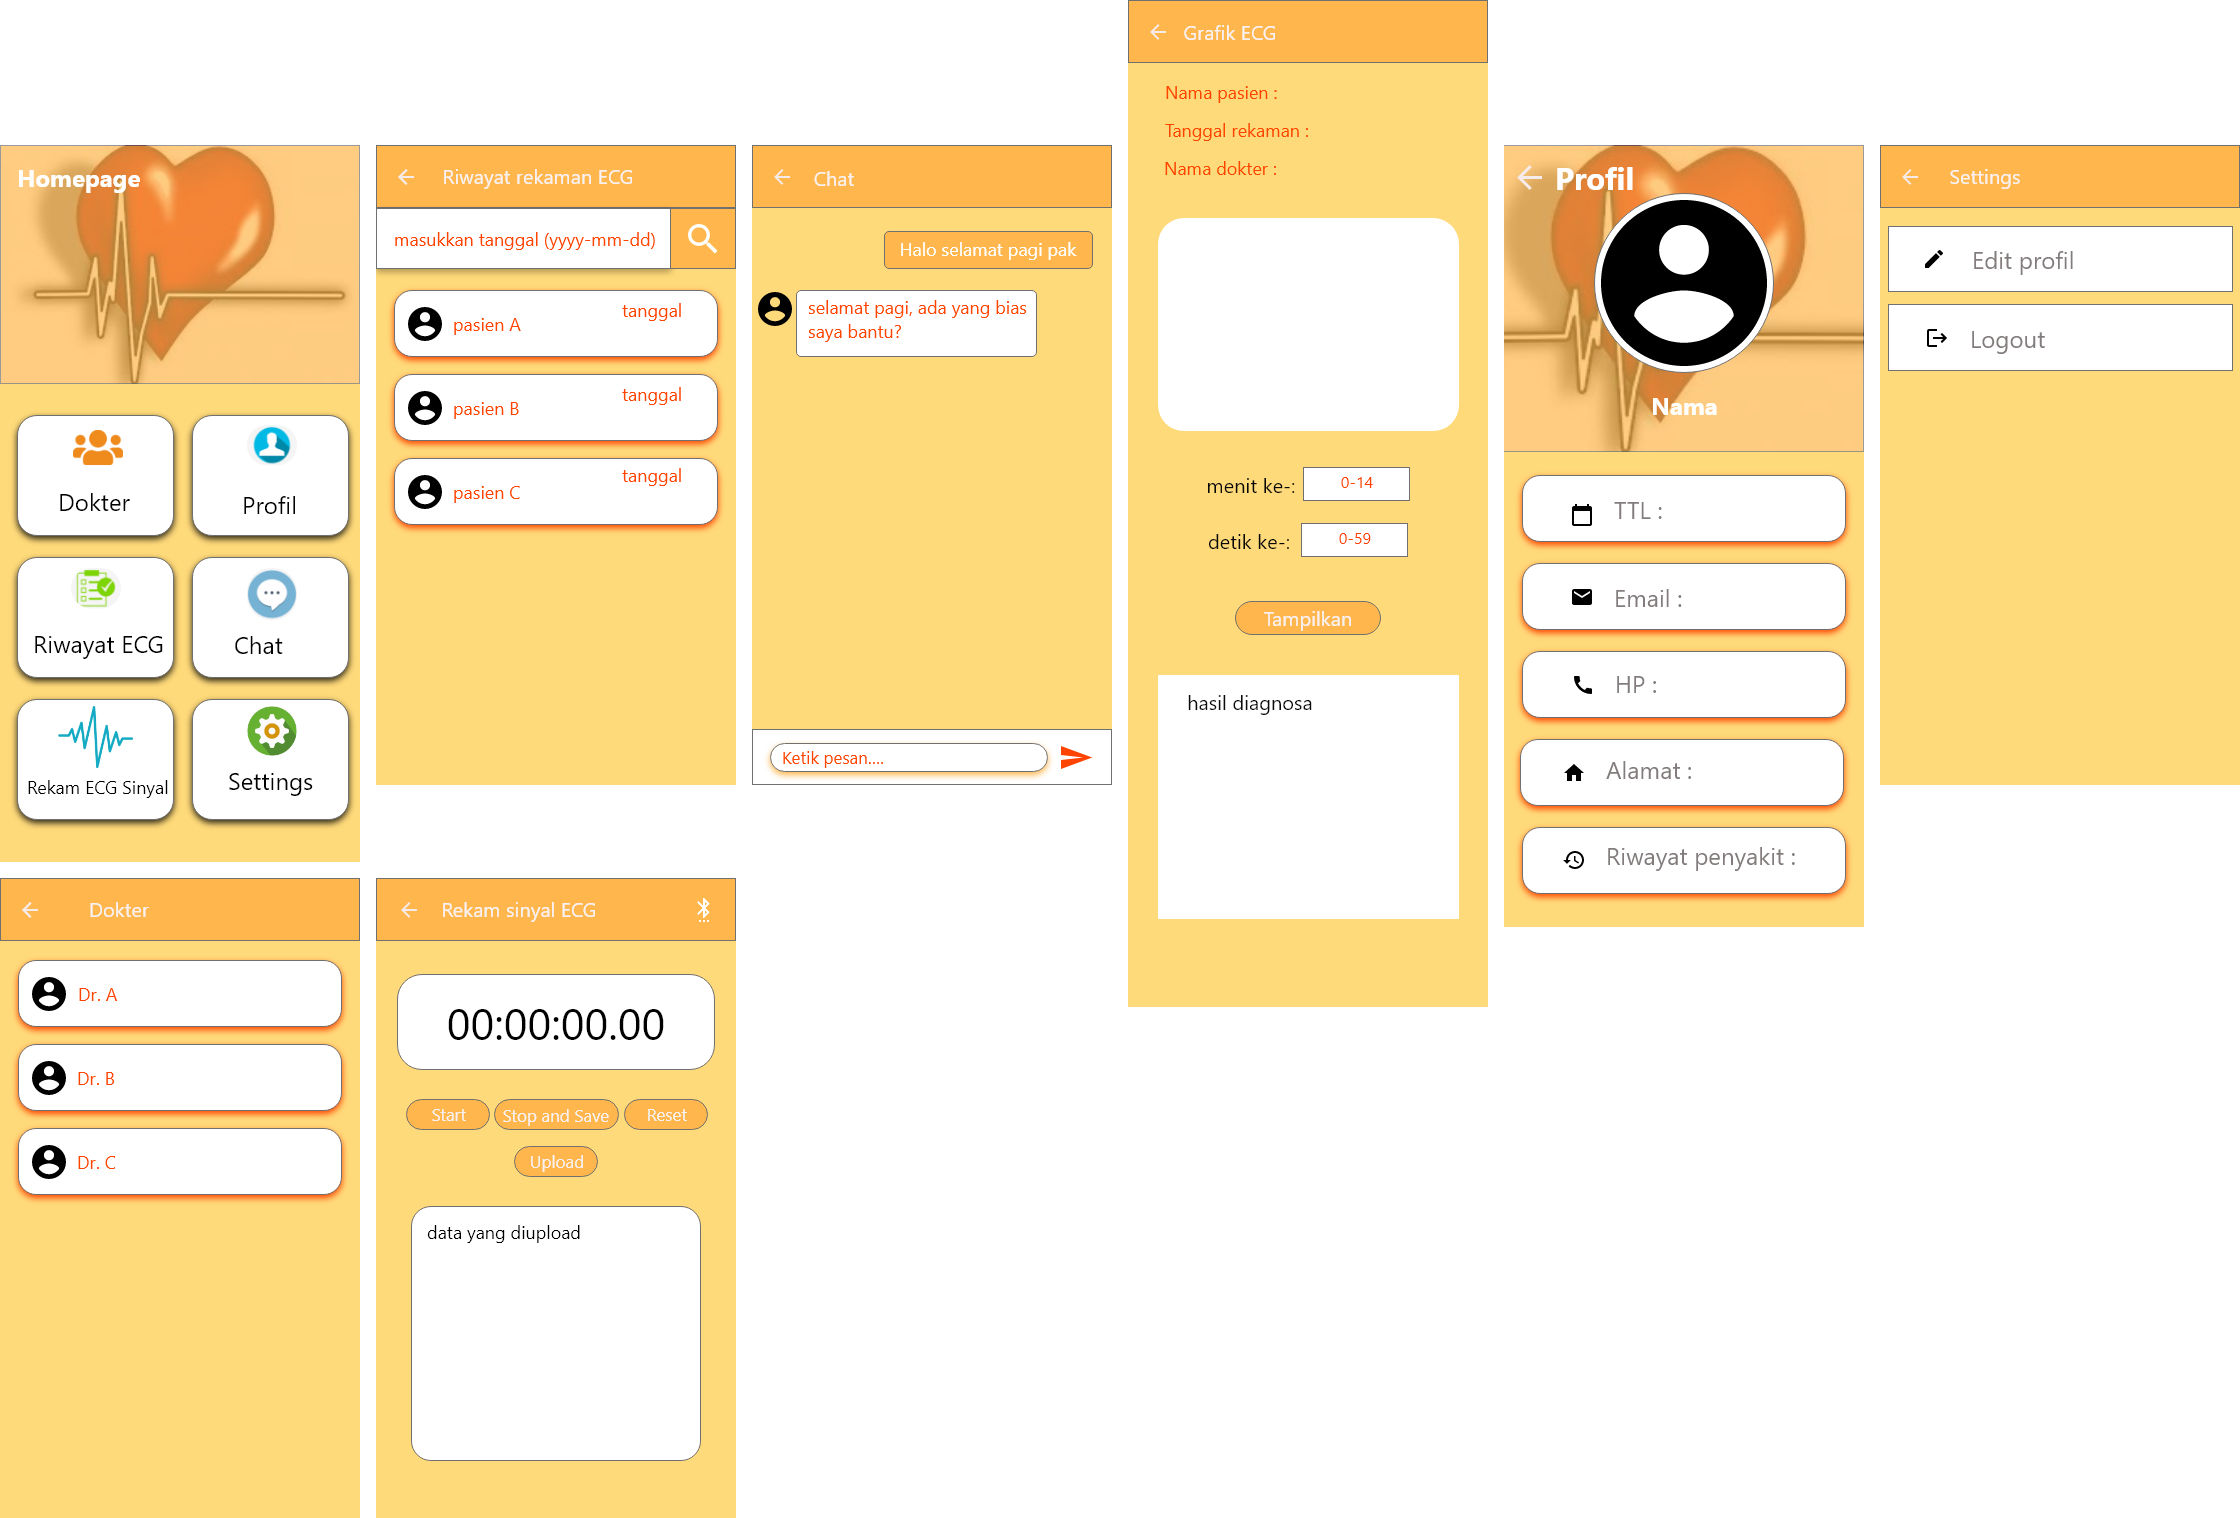
\includegraphics[width=1\textwidth]{img/pasienUI.png}
	\caption{Desain UI pada aplikasi pasien.}
	\label{fig:3.3}
\end{figure}
\vspace{1ex}
Dapat diketahui dari desai UI pasien tersebut terdapat 8 screen, yaitu:
\begin{enumerate}
	\vspace{-2mm}
	\item Homepage screen, yang mana merupakan halaman utaman pada aplikasi. Pada Homepage screen dokter tersedia 6 buah menu yaitu Dokter untuk berpindah menuju halaman daftar dokter yang ada, Profil untuk berpindah ke halaman profil, Chat untuk berpindah ke halaman chat, Riwayat ECG untuk berpindah halaman menuju riwayat rekaman ECG, Rekam ECG Sinyal untuk berpindah menuju halaman perekaman data ECG, dan Settings untuk berpindah ke halaman settings,
	\vspace{-2mm}
	\item Riwayat rekaman ECG screen yang sama seperti screen dokter, pada halaman ini pasien juga dapat mencari riwayat rekaman ECG pada waktu tertentu sesuai yang telah diinputkan,
	\vspace{-2mm}
	\item Chat screen, desain halaman chat untuk pasien juga sama seperti dokter,
	\vspace{-2mm}
	\item Grafik ECG screen, sama seperti dokter, pasien juga dapat melihat grafik ECG miliknya yang telah direkam. Pasien juga dapat melihat grafik pada menit dan detik tertentu. Pada halaman ini pasien juga dapat melihat hasil diagnosa yang telah ditambahkan oleh dokter,
	\vspace{-2mm}
	\item Profil screen, desain halaman profil untuk pasien juga sama seperti dokter. Pada halaman ini menampilkan informasi pasien yaitu foto, nama lengkap, tanggal lahir, email, nomor telepon, dan alamat,
	\vspace{-2mm}
	\item Settings screen, yang mana merupakan halaman yang berisi menu untuk mengubah informasi pada halaman profil dan juga terdapat menu \textit{logout} untuk keluar dari aplikasi.
	\vspace{-2mm}
	\item Dokter screen, yang mana merupakan menu tambahan untuk pasien. Pada halaman ini pasien dapat melihat daftar dokter yang ada dan melihat informasi profil dokter.
	\vspace{-2mm}
	\item Rekam sinyal ECG screen, yang mana merupakan halaman yang khusus untuk pasien. Pada halaman ini pasien dapat melakukan perekaman data ECG yang dikirim oleh arduino melalui bluetooth HC-05. Pada halaman ini terdapat icon bluetooth pada top bar yang mana berfungsi untuk menghubungkan bluetooth smartphone dengan modul HC-05. Halaman ini memiliki desain seperti stopwatch yang memiliki tombol start, stop, dan reset. Tombol start untuk memulai rekaman, stop untuk menghentikan rekaman sekaligus menyimpan data kedalam file.txt sementara, reset untuk mengembalikan ulang waktu stopwatch, dan terdapat tombol upload untuk mengupload data ke dalam database, data yang diupload dapat dilihat pada layar dibawahnya.
\end{enumerate}
\vspace{1ex}

Pada kedua gambar tersebut terdapat
sedikit perbedaan desain antara milik dokter dengan pasien. Perbedaan pertama desain tersebut terdapat pada jumlah menu di homepage. Pada desain UI homepage milik dokter memiliki menu yang lebih sedikit daripada pasien, hal ini dikarenakan dokter tidak perlu menggunakan fitur rekam sinyal sinyal dan juga fitur melihat dokter lain. Perbedaan kedua terdapat
pada layar grafik ECG yang berguna dapat menampilkan grafik sinyal jantung pada menit dan detik tertentu sesuai keinginan user.
Perbedaan pada layar grafik ECG adalah pada layar dokter
terdapat form dan tombol untuk menambahkan diagnosa sedangkan pada layar pasien hanya membutuhkan hasil diagnosa.

\vspace{1ex}

\section{Desain Database}
\vspace{1ex}

Pada penelitian ini menggunakan database MySQL. Berikut merupakan desain database pada penelitian ini ditunjukkan pada Gambar \ref{fig:3.4}. 
\begin{figure}[H] \centering
	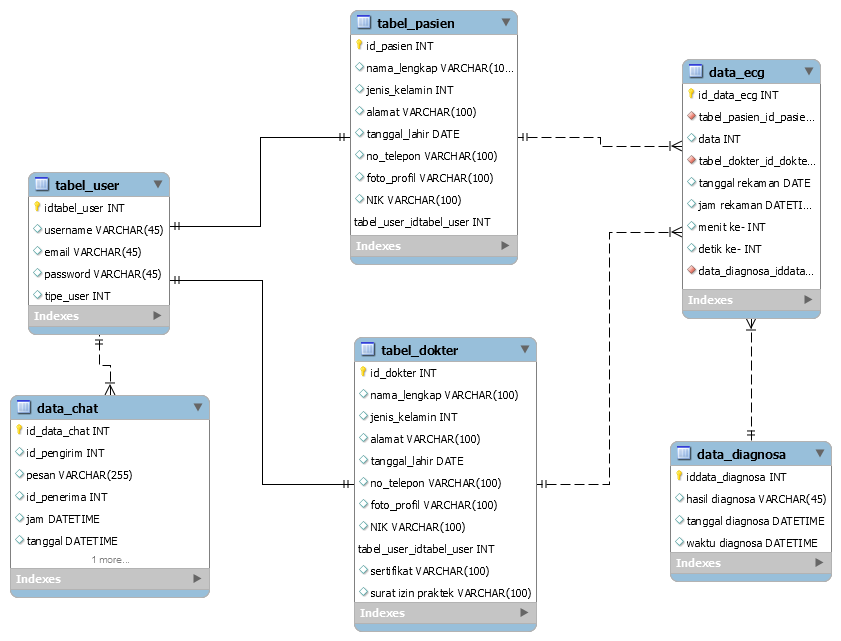
\includegraphics[width=1\textwidth]{img/db_revv.png}
	\caption{Desain database.}
	\label{fig:3.4}
\end{figure}
\vspace{1ex}

Dalam database terdapat 6 tabel yang diperlukan untuk menyimpan masing-masing data, yaitu:
\begin{enumerate}[nolistsep]
	\item Tabel tabel\_user, memiliki 5 kolom. Tabel user digunakan sebagai tempat menyimpan data login pengguna aplikasi yaitu username, email, password, dan tipe user untuk lebih mudah membedakan antara data pasien dan dokter. Tabel user memiliki relasi dengan 3 tabel lainnya yaitu tabel pasien, tabel dokter, dan tabel data \textit{chat}.
	\item Tabel tabel\_pasien, memiliki 9 kolom dengan 1 kolom merupakan \textit{foreign key} dari tabel user. Tabel pasien digunakan sebagai tempat menyimpan data pasien berupa id pasien, nama lengkap, jenis kelamin, alamat, tanggal lahir, NIK, nomor telepon, foto profil , dan id user yang merupakan \textit{foreign key} dari tabel user. Tabel pasien memiliki 2 relasi dengan 2 tabel lainnya yaitu tabel user dan tabel data ECG.
	\item Tabel tabel\_dokter, memiliki 11 kolom  dengan 1 kolom merupakan \textit{foreign key} dari tabel user. Tabel dokter digunakan sebagai tempat menyimpan data dokter berupa id dokter, nama lengkap, jenis kelamin, alamat, tanggal lahir, NIK, nomor telepon, foto profil, sertifikat, surat izin praktek, dan id user yang merupakan \textit{foreign key} dari tabel user. Tabel dokter memiliki 2 relasi dengan 2 tabel lainnya yaitu tabel user dan tabel data ECG.  
	\item Tabel data\_ecg, memiliki 9 kolom, 3 kolom merupakan foreign key dari tabel pasien, tabel dokter, dan tabel data\_diagnosa. Tabel data\_ecg digunakan untuk menyimpan data rekaman sinyal jantung pasien yang mana akan dapat ditampilkan pada aplikasi android. Tabel data ECG terdiri dari kolom id\_data\_ecg, id\_pasien yang merupakan \textit{foreign key} dari tabel\_pasien, data, id\_dokter yang merupakan \textit{foreign key} dari tabel\_dokter, tanggal rekaman, jam rekaman, jam, menit, detik, dan id\_data\_diagnosa yang merupakan \textit{foreign key} dari tabel data diagnosa.
	\item Tabel data\_diagnosa, memiliki 4 kolom, Tabel ini digunakan sebagai tempat penyimpanan hasil diagnosa yang telah ditambahkan oleh dokter. Tabel data diagnosa memiliki relasi dengan tabel data ecg. Tabel ini terdiri dari kolom id\_data\_diagnosa, hasil diagnosa, tanggal diagnosa, dan waktu diagnosa.		
	\item Dan tabel data\_chat yang memiliki 6 kolom. Tabel data\_chat diperlukan untuk menyimpan data chat antara pasien dan dokter. Tabel ini terdiri dari kolom id\_data\_chat, id\_pengirim, pesan, id\_penerima, jam, dan tanggal. Tabel data\_chat memiliki relasi dengan tabel tabel\_user.
\end{enumerate}

\section{Akuisisi Data}
\vspace{1ex}

Akuisisi data pada penelitian ini menggunakan sensor ECG AD8232. Setelah sensor AD8232 membaca sinyal jantung pasien, kemudian data sinyal jantung akan diproses pada mikrokontroler arduino. Setelah data sinyal diproses oleh arduino, data sinyal akan dikirimkan melalui serial bluetooth HC-05. \textit{Baudrate} yang digunakan pada modul bluetooth HC-05 adalah 57600. Data sinyal ECG yang dikirimkan pada aplikasi android akan disimpan sementara pada file.txt. Akuisisi data yang dilakukan pada penelitian ini adalah sebesar kurang lebih 128 Hz atau 128 data sampel sinyal tiap detik. Berikut merupakan perangkat ECG yang digunakan, ditunjukkan pada gambar \ref{fig:3.4.1}.
\begin{figure}[H] \centering
	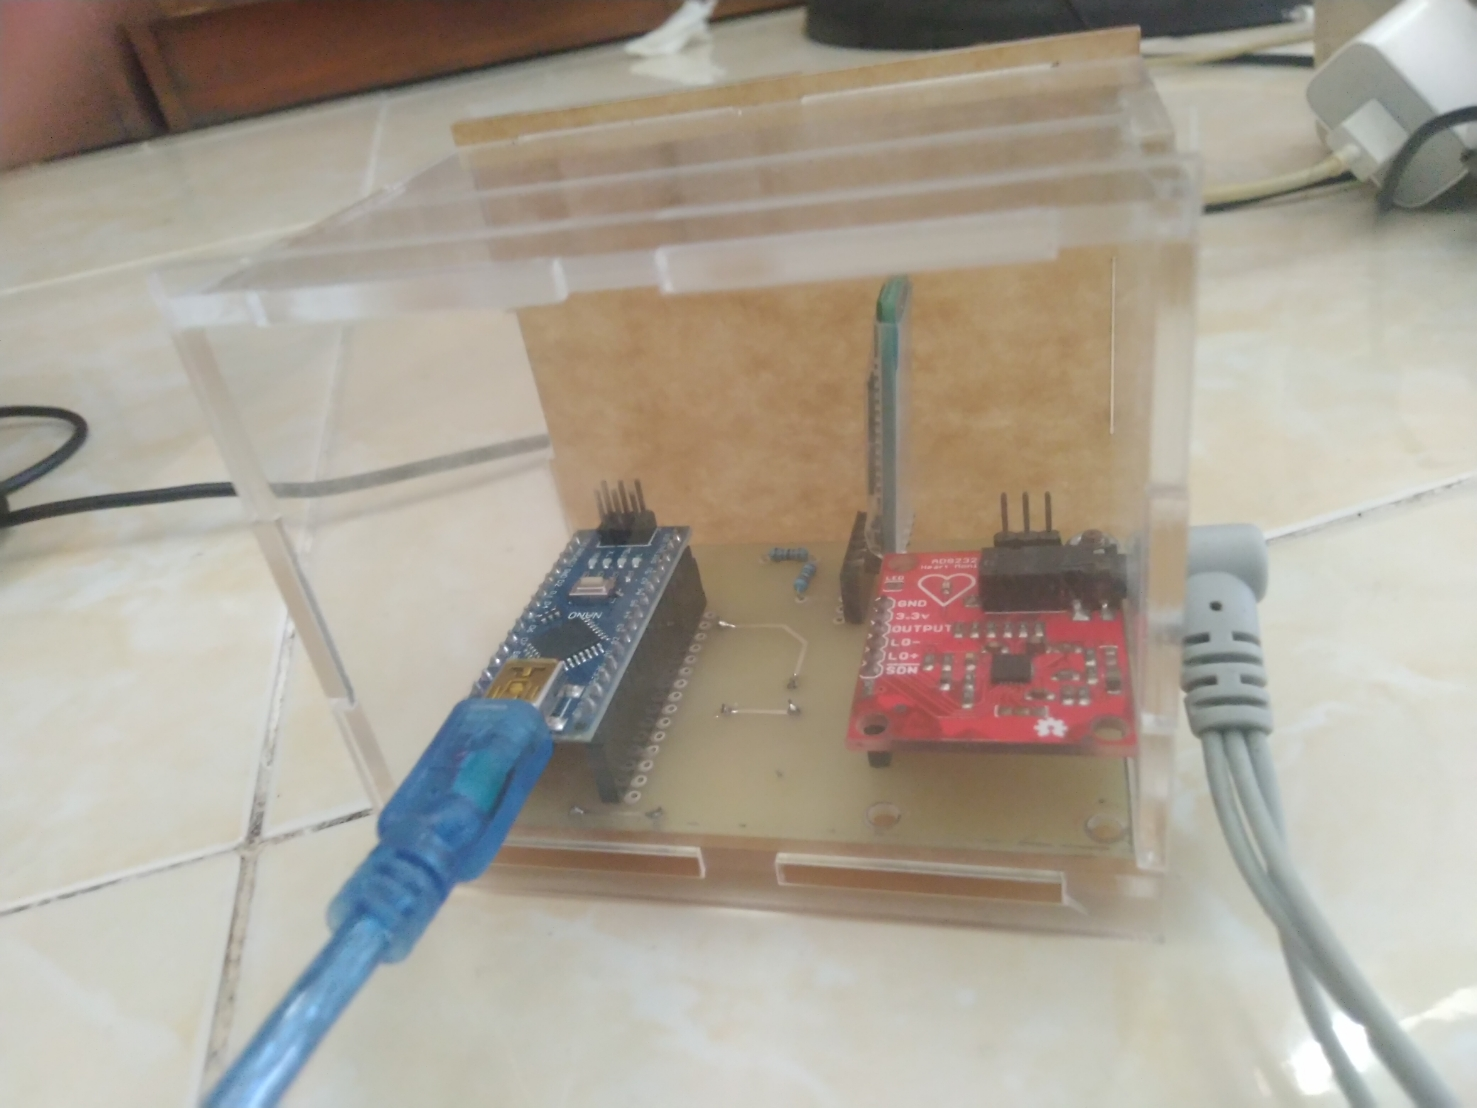
\includegraphics[width=0.6\textwidth]{img/fotoperangkat1.jpg}
	\caption{Perangkat ECG.}
	\label{fig:3.4.1}
\end{figure}
\vspace{1ex}

Mekanisme kerja pada akuisisi data adalah modul Bluetooth menunggu perintah dari aplikasi, kemudian aplikasi memberi perintah angka "1" yang mana berarti meminta alat mulai mengambil data. Disaat arduino menerima perintah "1" dari HC-05, arduino mulai melakukan looping mengambil data dari sensor AD8232. Apabila waktu rekaman sudah berjalan selama 15 menit, aplikasi akan mengirim perintah angka "0" pada HC-05 yang mana berarti untuk menghentikan rekaman. Pada saat arduino menerima perintah "0" dari HC-05, maka arduino akan berhenti melakukan looping untuk mengambil data. Berikut merupakan gambar diagram mekanisme kerja akuisisi data Gambar \ref{fig:3.4.2}.
\begin{figure}[H] \centering
	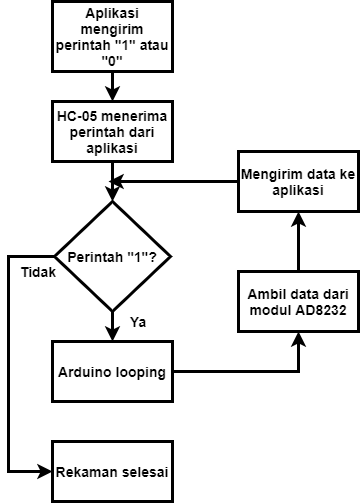
\includegraphics[width=0.6\textwidth]{img/diagramAkuisisi.png}
	\caption{Diagram mekanisme akuisisi data.}
	\label{fig:3.4.2}
\end{figure}


\section{Perekaman Data}
\vspace{1ex}
Perekaman data dilakukan oleh aplikasi android. Proses rekaman pada pasien adalam kurang dari sampai dengan 15 menit. Berikut merupakan implementasi halaman rekaman data pada aplikasi android ditunjukkan oleh Gambar \ref{fig:3.5}.

\begin{figure}[H] \centering
	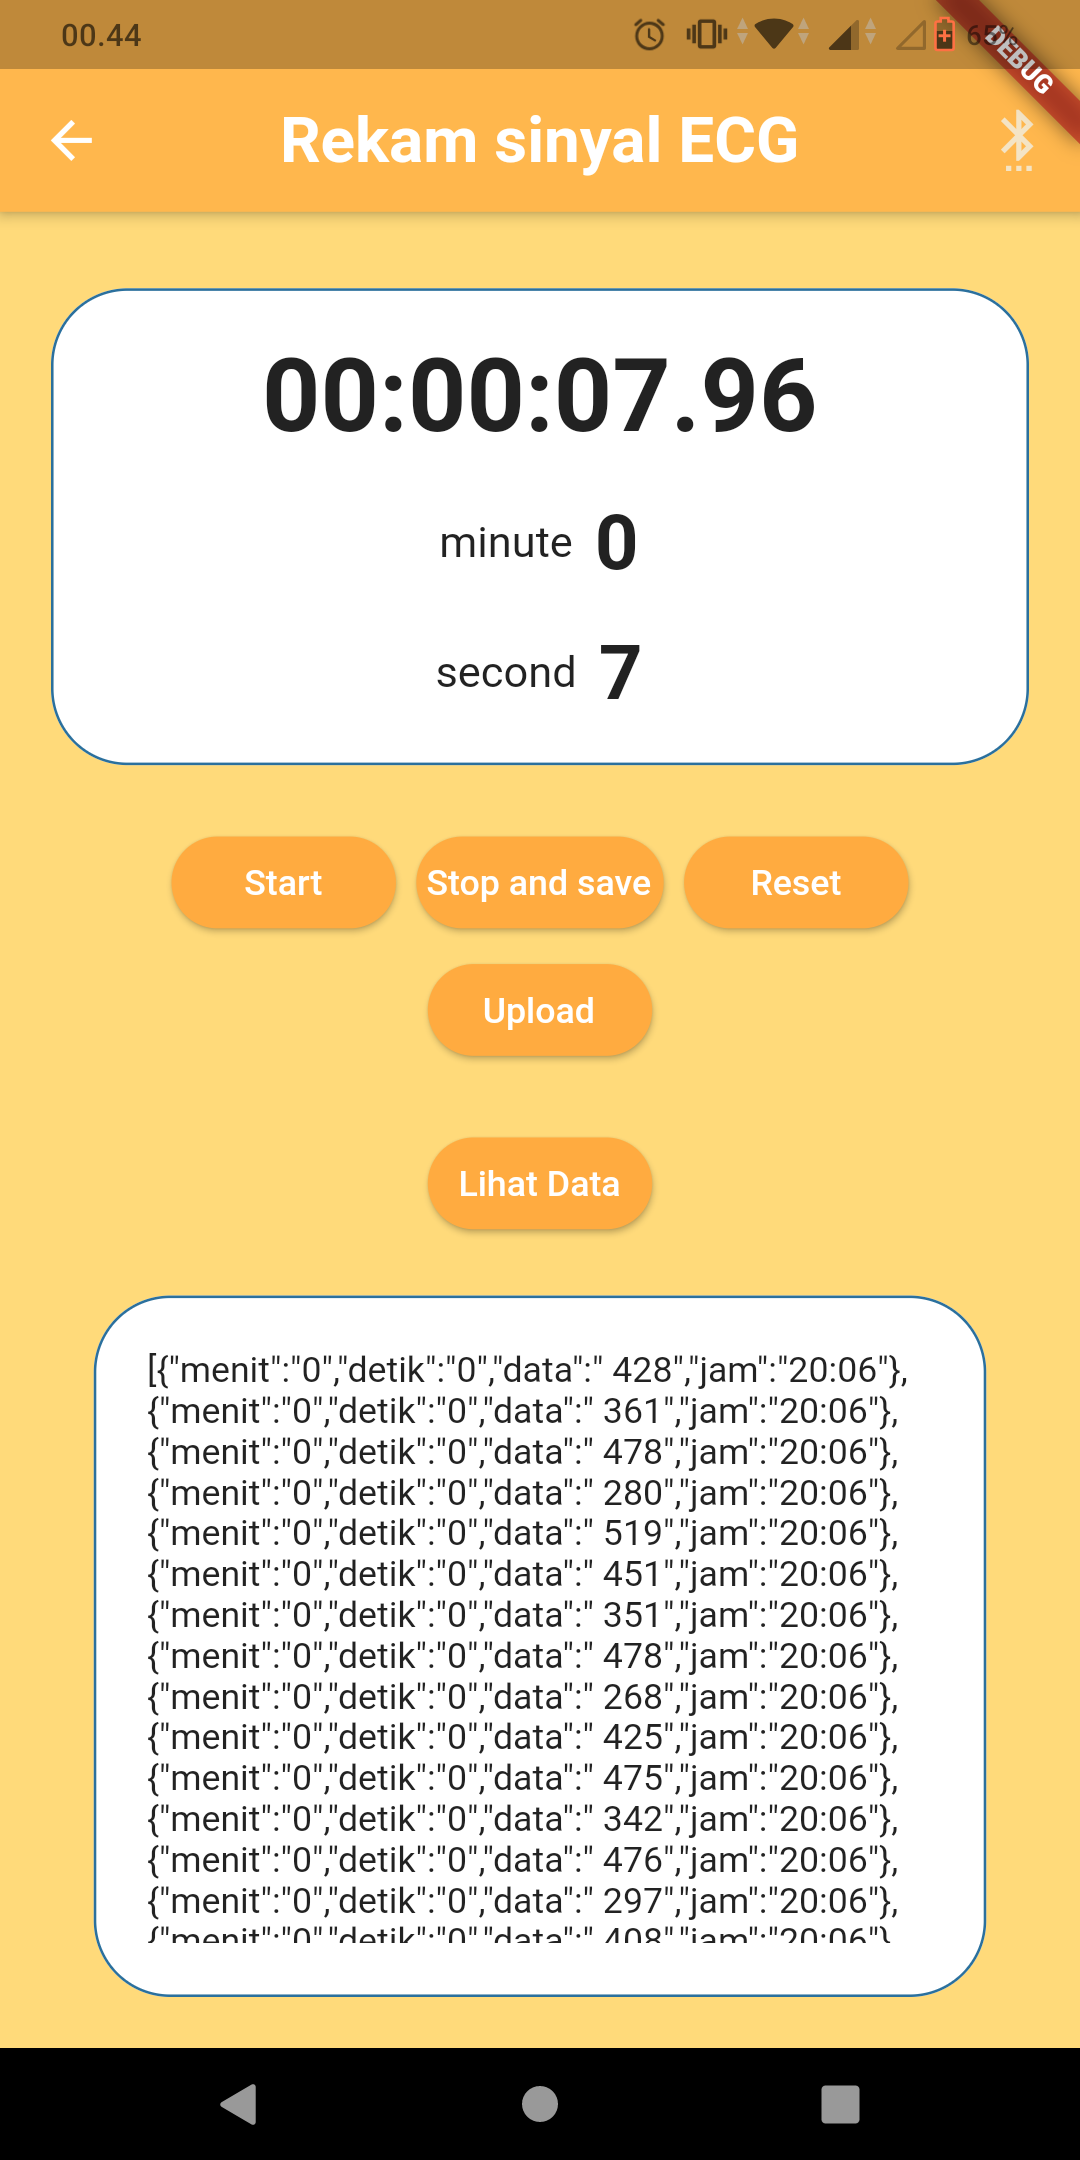
\includegraphics[width=0.37\textwidth]{img/layar_rekaman.png}
	\caption{Implementasi UI Rekam Sinyal ECG.}
	\label{fig:3.5}
\end{figure}


Selama proses rekaman berlangsung, aplikasi akan menerima data sinyal terus-menerus dari modul bluetooth HC-05. Aplikasi akan menyimpan data sinyal kedalam string saat proses rekaman berlangsung. Setelah rekaman selesai, aplikasi akan menyimpan data sinyal dari variabel string kedalam file.txt. Dapat dilihat pada layar rekaman (Gambar \ref{fig:3.5}) terdapat stopwatch untuk mengetahui seberapa lama telah melakukan rekaman. Pada layar ini terdapat 4 tombol, yaitu tombol Start yang berfungsi untuk memulai rekaman, Stop and Save berfungsi untuk menghentikan rekaman dan menyimpan data dalam file.txt, tombol Reset berfungsi untuk mengembalikan stopwatch dengan keadaan waktu 00:00:00.00, tombol Upload yang berguna untuk mengupload data sinyal menuju database, dan yang terakhir adalah tombol Lihat Data yang berguna untuk menampilkan isi dari file.txt. Isi file.txt ditampilkan pada box putih seperti yang tertera dibawah tomboh Lihat Data.

\vspace{1ex} 
\section{Penyimpanan Data}
\vspace{1ex}
Data rekaman sinyal  ECG yang diupload oleh aplikasi pada database disimpan dalam tabel data\_ecg. Data ECG disimpan beserta atribut lainnya sesuai kolom yang ada pada tabel data\_ecg. Rincian kolom tersebut sebagai berikut:
\begin{enumerate}
	\vspace{-2mm}
	\item Kolom id\_data\_ecg dengan tipe data BIGINT sebagai primary key dan auto increment untuk menyimpan nomor urut data ECG yang didapat,
	\vspace{-2mm}
	\item Kolom id\_pasien dengan tipe data INT untuk menyimpan id pasien,
	\vspace{-2mm}
	\item Kolom data dengan tipe data INT berguna untuk menyimpan data ECG hasil rekaman,
	\vspace{-2mm}
	\item Kolom menit dengan tipe data INT untuk menyimpan waktu menit,
	\vspace{-2mm}
	\item Kolom detik dengan tipe data INT untuk menyimpan waktu detik,
	\vspace{-2mm}
	\item Kolom id\_dokter dengan tipe data INT untuk menyimpan id dokter,
	\vspace{-2mm}
	\item Kolom tanggal dengan tipe data DATE berguna untuk menyimpan data tanggal rekaman,
	\vspace{-2mm}
	\item Kolom jam dengan tipe data VARCHAR untuk menyimpan nomor sample data pada waktu mulai rekaman sampai akhir rekaman, (data ini digunakan sebagai sumbu X untuk menggambarkan grafik pada aplikasi),
	\vspace{-2mm}
	\item Kolom channel dengan tipe data INT berfungsi untuk menyimpan channel lead ECG,
	\vspace{-2mm}
	\item Kolom clock dengan tipe data VARCHAR untuk menyimpan waktu mulai rekaman,
	\vspace{-2mm}
	\item Kolom id\_data\_diagnosa dengan tipe data INT untuk menyimpan nomor id diagnosa dari tabel data\_diagnosa,
\end{enumerate}

Berikut merupakan potongan database pada tabel data\_ecg yang ditunjukkan pada Gambar  \ref{fig:3.6}.

\begin{figure}[H] \centering
	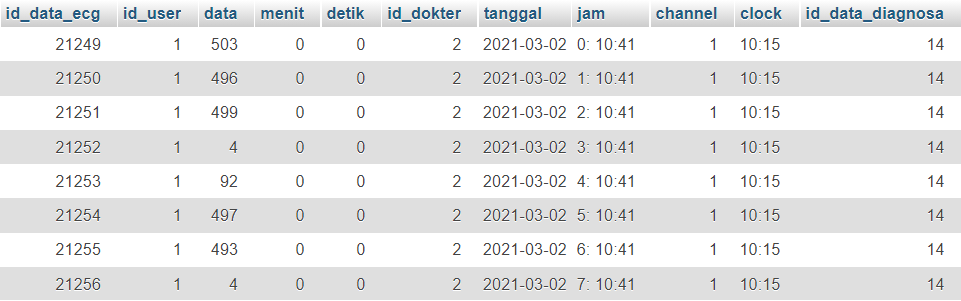
\includegraphics[width=1\textwidth]{img/tabel data ecg.png}
	\caption{Tabel data\_ecg.}
	\label{fig:3.6}
\end{figure}

\vspace{1ex} 
\section{Menampilkan Data}
\vspace{1ex}

Data yang telah disimpan pada database yaitu dalam tabel data\_ecg dapat diambil oleh aplikasi dokter dan pasien untuk ditampilkan dalam bentuk grafik. Pada screen grafik ECG, pengguna dapat melihat data ECG sesuai dengan waktu yang ditentukan yaitu pada (menit awal, detik awal) sampai dengan (menit akhir, detik akhir) dengan selisih waktu detik yang dapat diatur pada box (parameter range). Pengguna juga dapat melihat data selanjutnya dengan menekan tombol "selanjutnya" serta dapat kembali ke data sebelumnya dengan menakan tombol "sebelumnya". Berikut adalah tampilan dari screen Grafik sinyal ECG dokter ditunjukkan pada Gambar \ref{fig:3.7}. 

\begin{figure}[H] \centering
	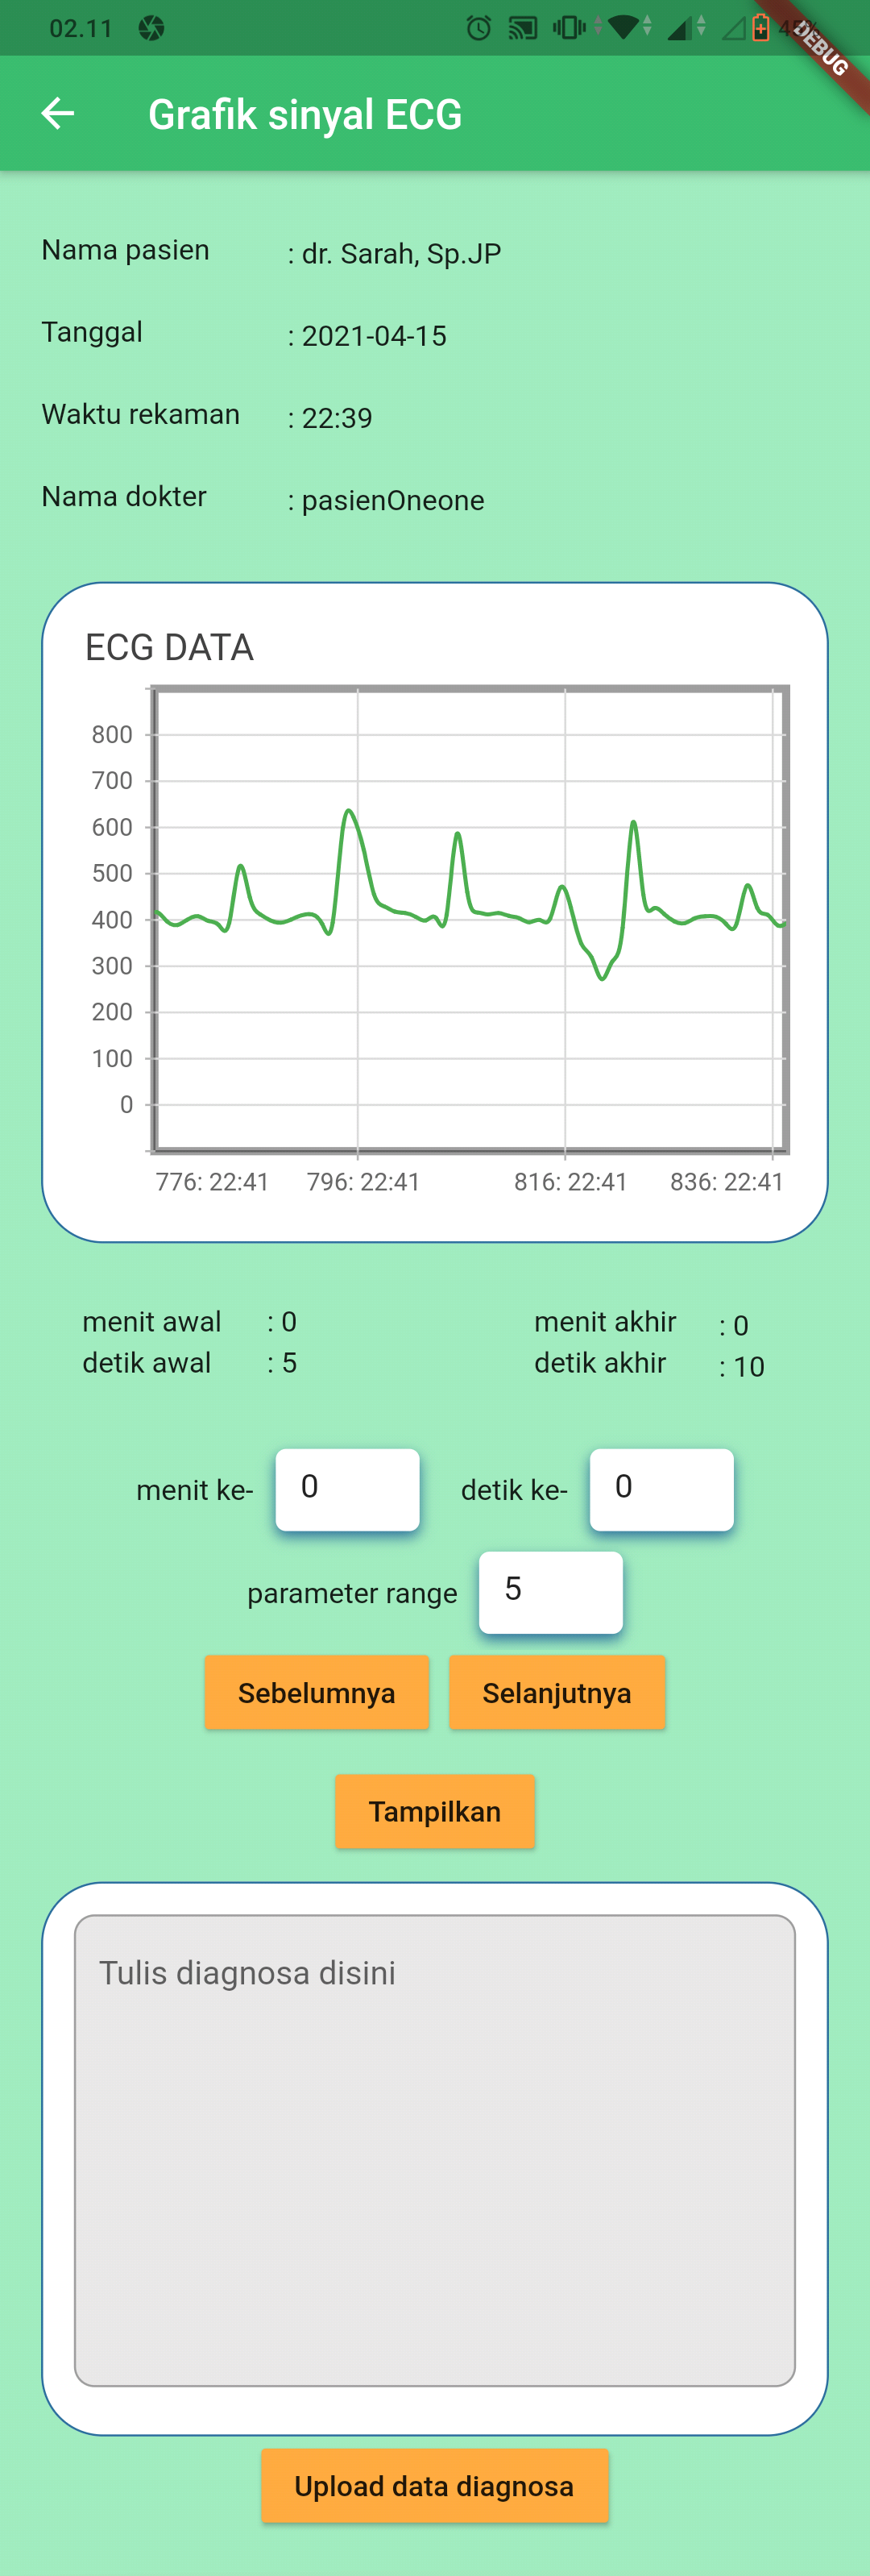
\includegraphics[width=0.4\textwidth]{img/layar_grafikECGdokter.png}
	\caption{Implementasi UI Grafik ECG dokter.}
	\label{fig:3.7}
\end{figure}

Pada grafik tersebut terdiri dari sumbu X dan sumbu Y. Sumbu X merupakan data ECG yang diambil dari kolom data pada tabel data\_ecg, sedangkan sumbu Y merupakan data dari kolom jam pada tabel data\_ecg (Gambar \ref{fig:3.6}). Untuk tampilan Grafik sinyal ECG pasien tidak jauh berbeda. Berikut adalah tampilan dari screen Grafik sinyal ECG pasien ditunjukkan pada Gambar \ref{fig:3.8}.

\begin{figure}[H] \centering
	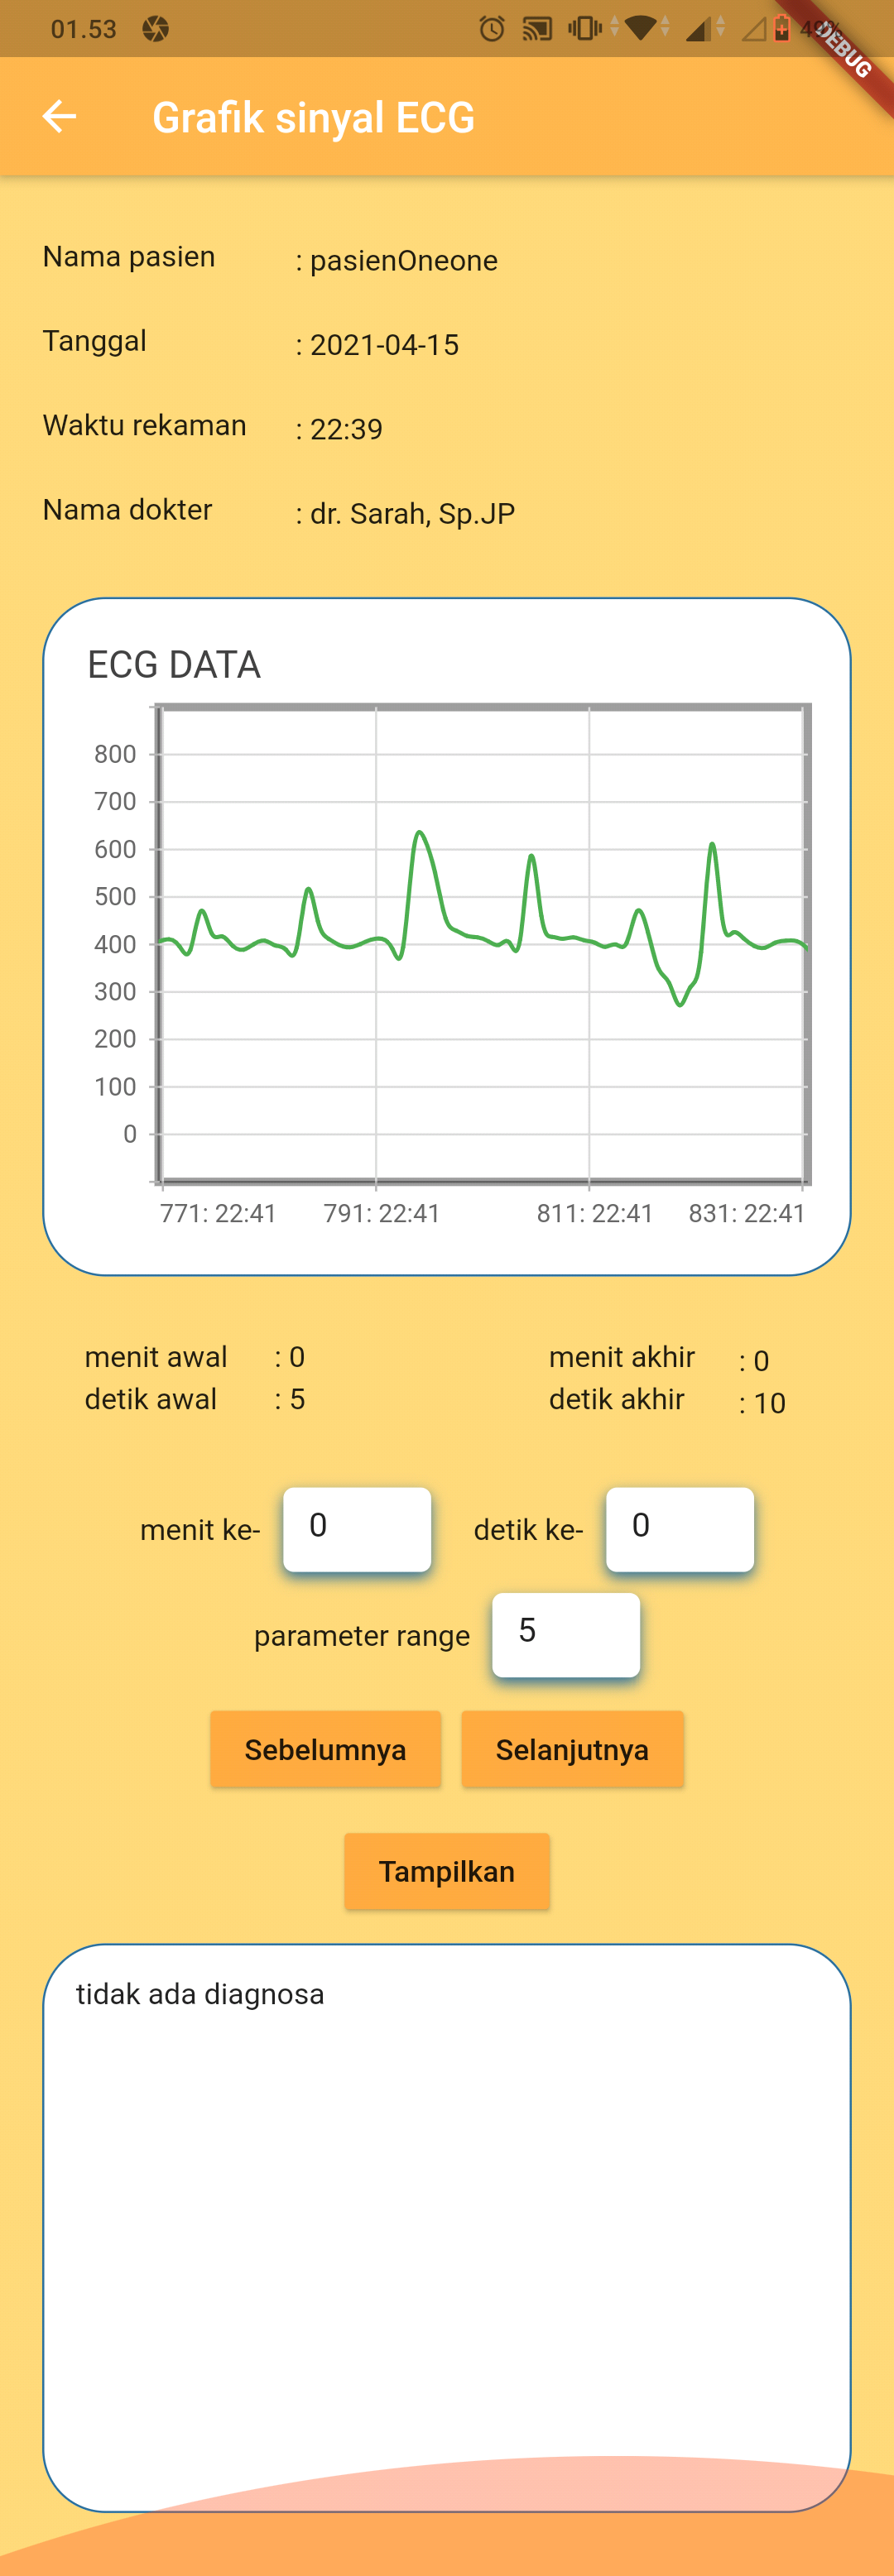
\includegraphics[width=0.4\textwidth]{img/layar_grafikECGpasien.png}
	\caption{Implementasi UI Grafik ECG pasien.}
	\label{fig:3.8}
\end{figure}

Dapat dilihat pada screen dokter (Gambar \ref{fig:3.7}) terdapat box berwarna abu-abu dengan keterangan "Tulis diagnosa disini" yang berarti pada screen dokter dapat ditambahkan diagnosa melalui box tersebut dan kemudian diupload dengan cara menekan tombol "Upload data diagnosa". Sedang kan pada screen pasien (Gambar \ref{fig:3.8}) hanya terdapat box putih tanpa ada tombol upload data diagnosa. Box putih tersebut adalah tempat hasil diagnosa yang diberikan oleh dokter.

\vspace{1ex} 
\section{Diagnosa Data}
\vspace{1ex}

Diagnosa sinyal ECG dilakukan secara manual yaitu oleh dokter. Dokter dapat menambahkan diagnosa pada rekaman ECG pasien dimenit dan detik tertentu, dapat dilihat pada Gambar \ref{fig:3.7} sebelumnya. Pada screen tersebut terdapat box untuk dokter yang berfungsi untuk tempat menambahkan diagnosa. Setelah dokter selesai menambahkan diagnosa, kemudian dapat mengupload ke database melalui tombol "Upload data diagnosa". Diagnosa yang telah diupload ke database akan disimpan pada tabel data\_diagnosa. Kemudian data diagnosa dapat ditampilkan pada aplikasi smarftphone pasien seperti yang ditunjukkan Gambar \ref{fig:3.9}.

\begin{figure}[H] \centering
	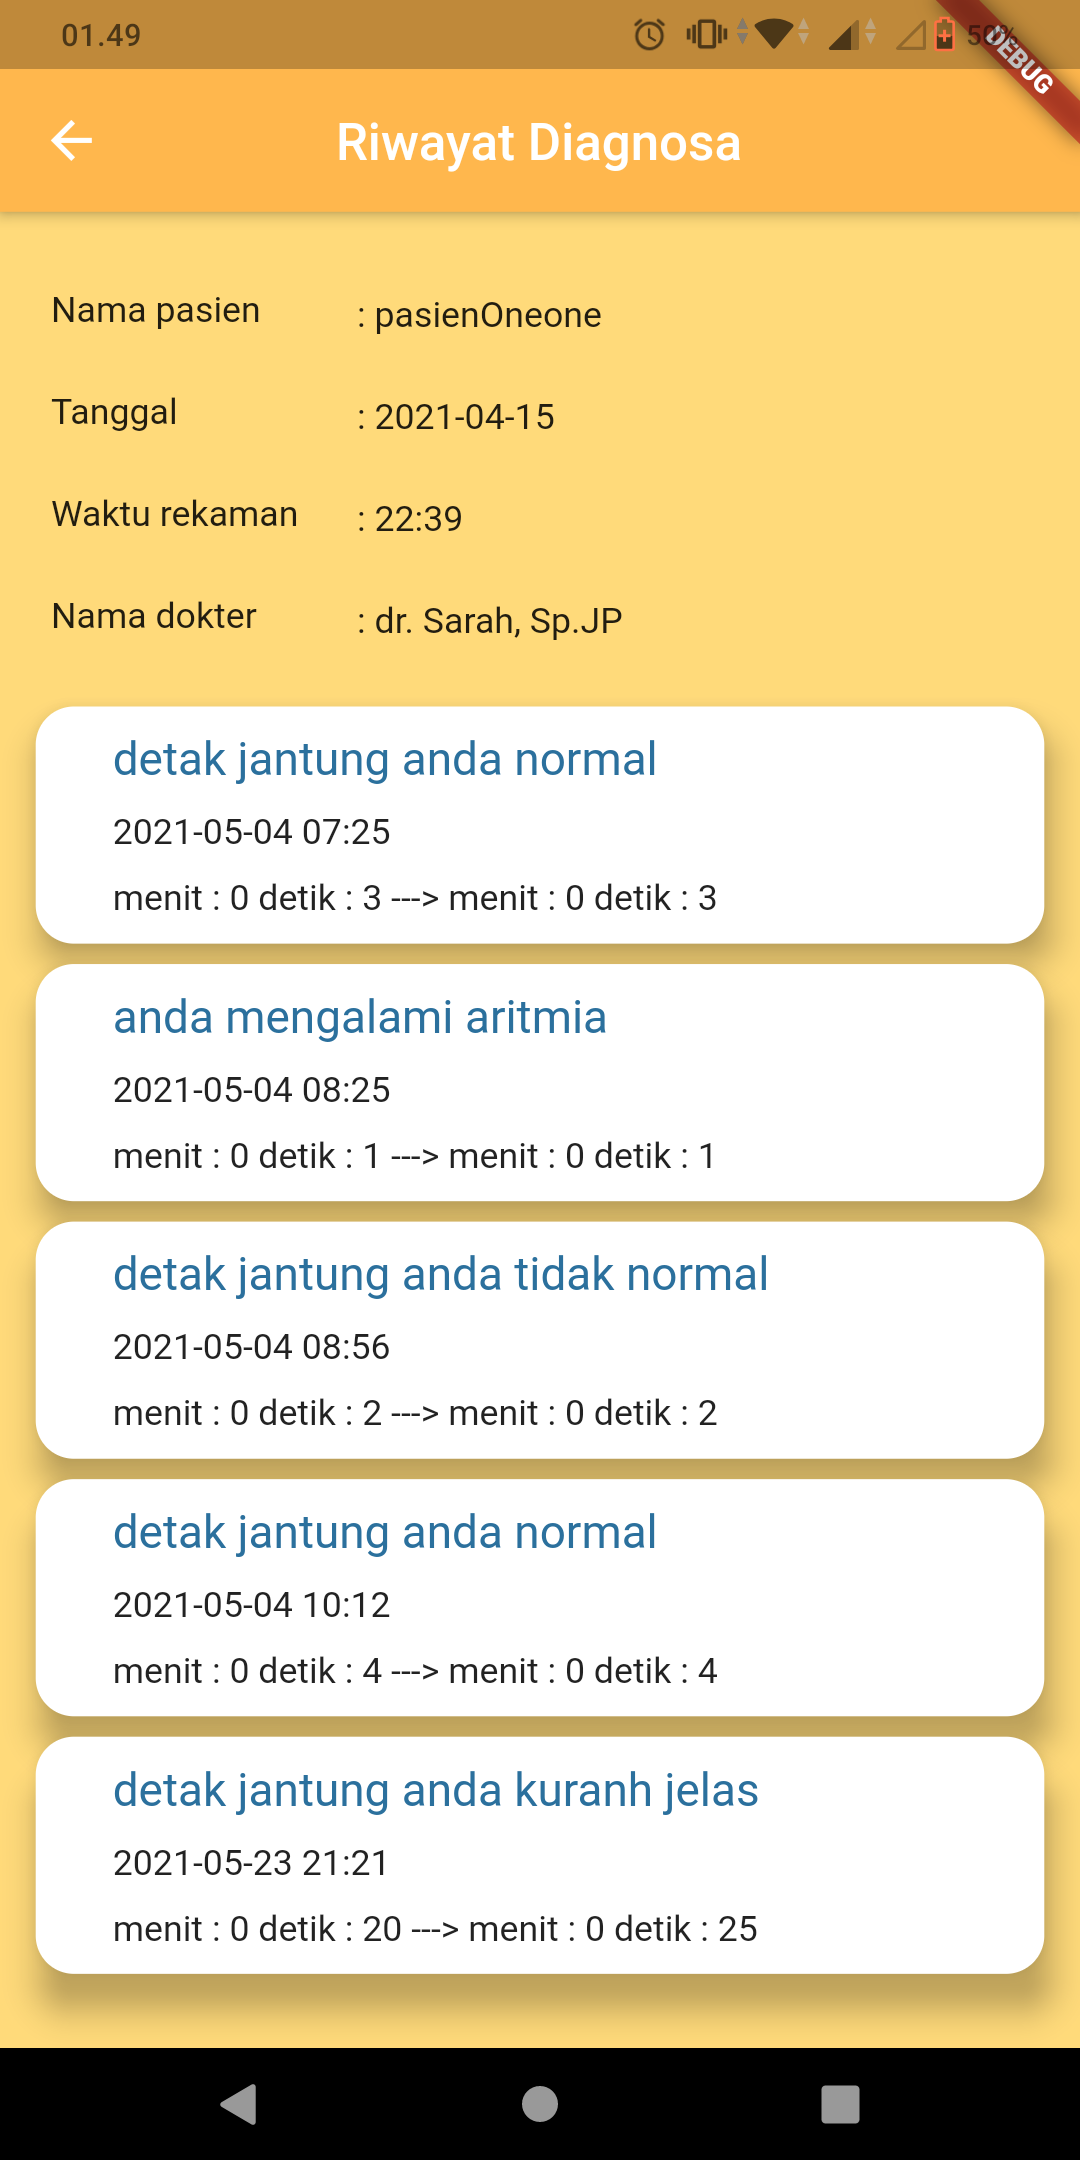
\includegraphics[width=0.4\textwidth]{img/layar_riwayatdiagnosa.png}
	\caption{Implementasi UI Riwayat Diagnosa.}
	\label{fig:3.9}
\end{figure}

\vspace{1ex}
\section{Fitur Chat}
\vspace{1ex}

Pada aplikasi ini tersedia fitur chat agar pasien dapat berkonsultasi dengan dokter spesialis. Untuk cara kerja pada screen chat ini, aplikasi akan melakukan refresh setiap detik dan akan mengambil data dari database yaitu pada tabel data\_chat agar pesan terbaru pada screen chat dapat muncul. Saat mengirim pesan, pesan dari kedua user pasangan chat akan diupload pada tabel yang sama. Untuk membedakannya terdapat pada kolom id\_pengirim dan id\_penerima yang terdapat pada tabel data\_chat (Gambar \ref{fig:3.6}). Tampilan screen chat pasien dapat dilihat pada Gambar \ref{fig:3.10}.

\begin{figure}[H] \centering
	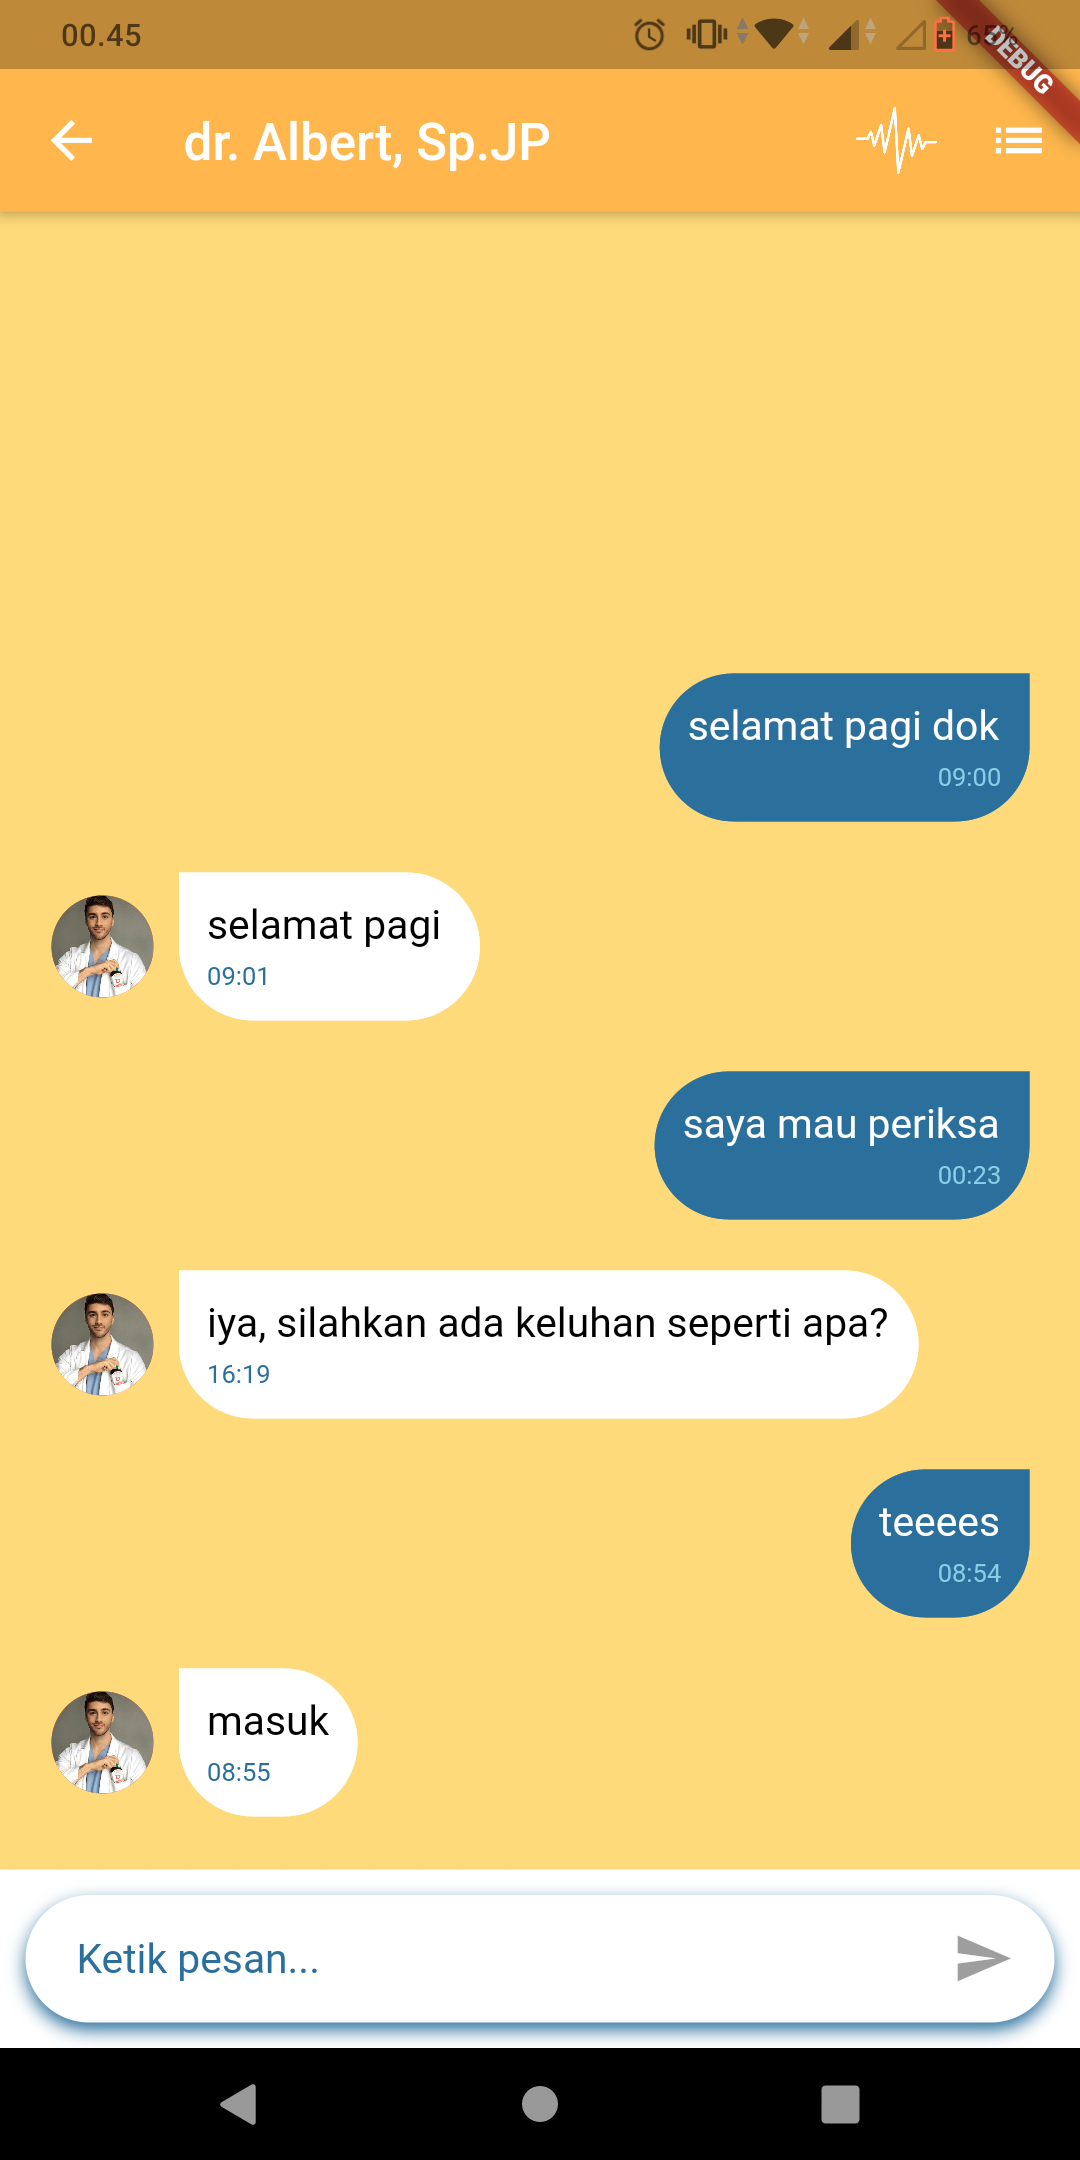
\includegraphics[width=0.4\textwidth]{img/layar_chatpasien.png}
	\caption{Implementasi UI Chatscreen Pasien.}
	\label{fig:3.10}
\end{figure}

Sedangkan untuk tampilan screen chat dokter dapat dilihat pada Gambar \ref{fig:3.11}.

\begin{figure}[H] \centering
	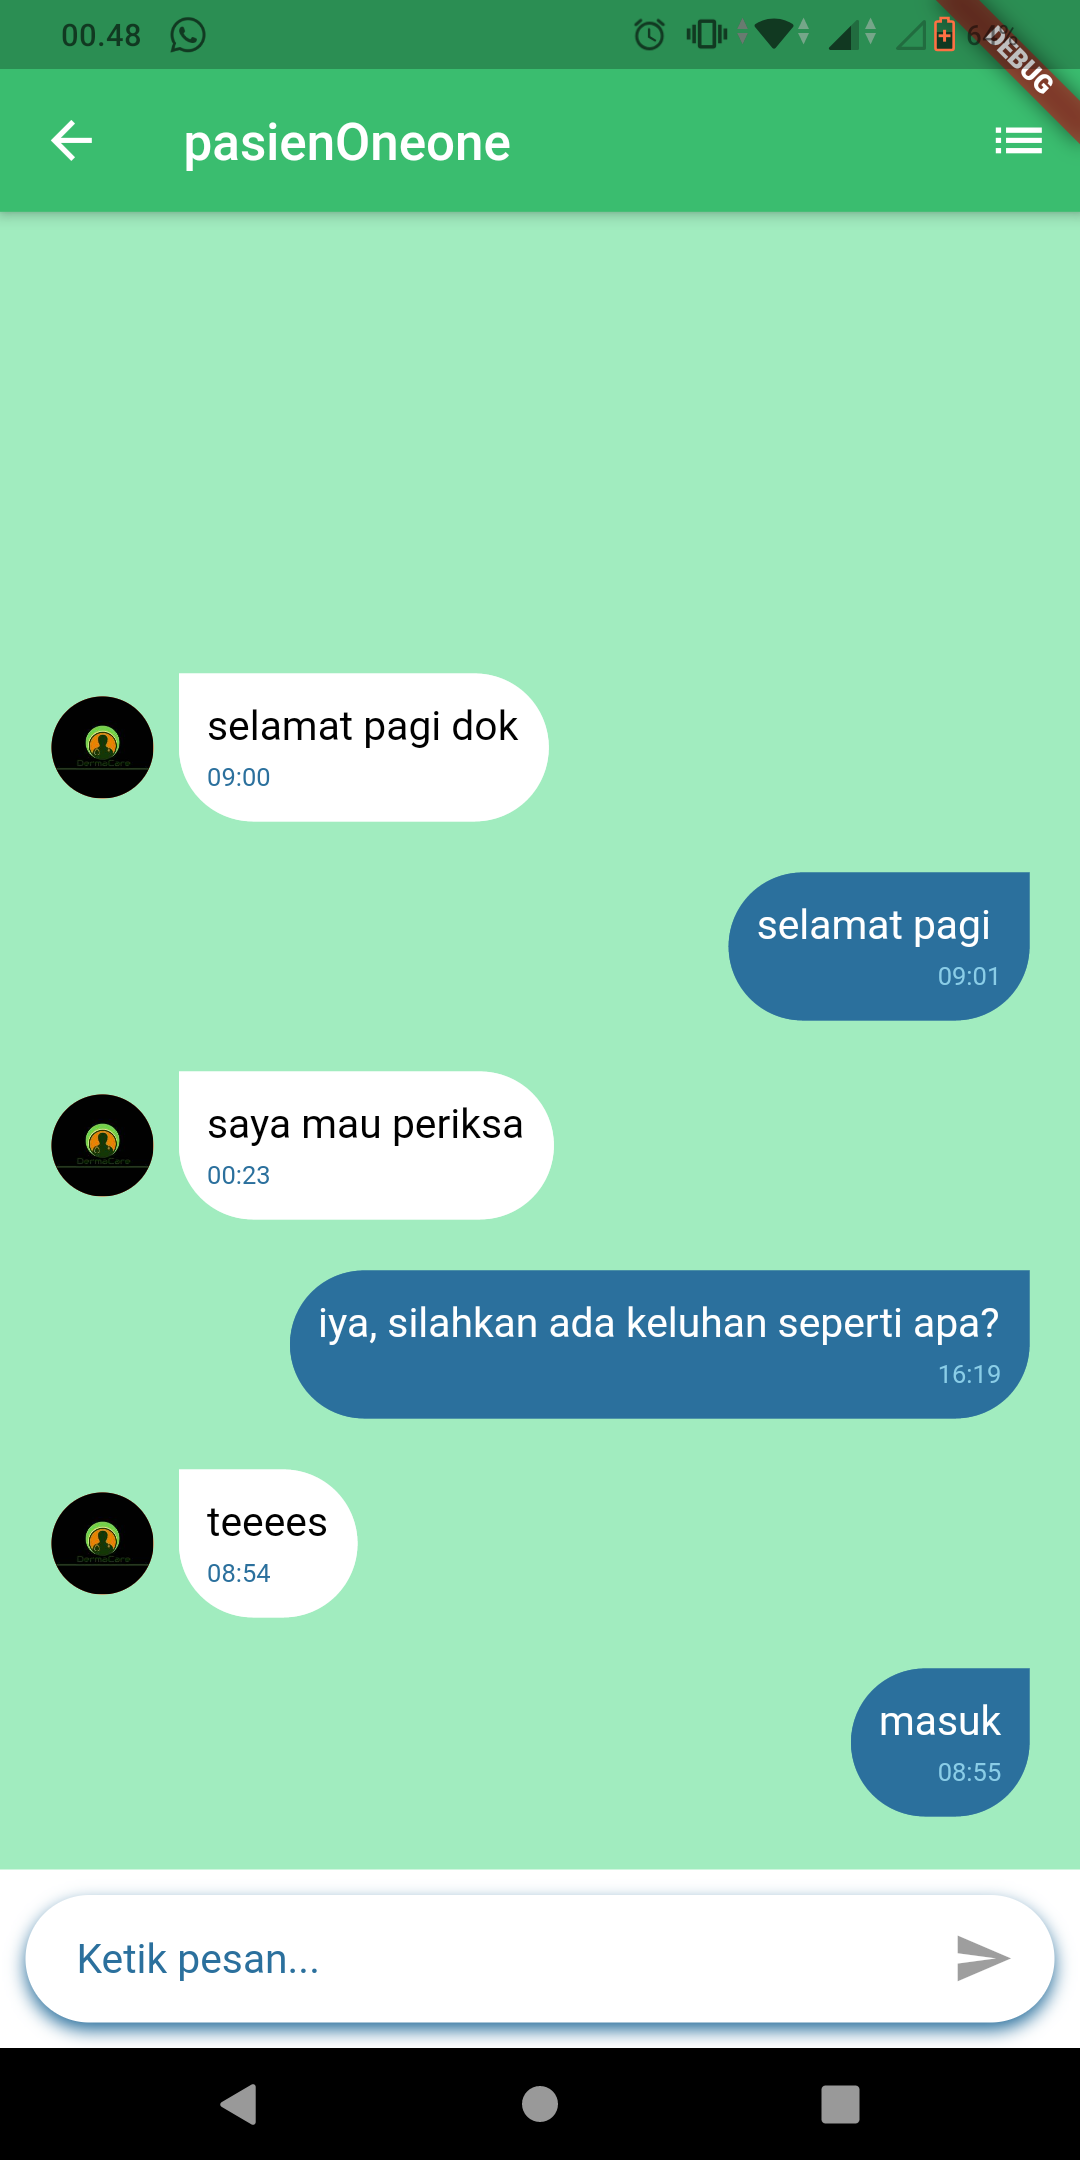
\includegraphics[width=0.4\textwidth]{img/layar_chatdokter.png}
	\caption{Implementasi UI Chatscreen Dokter.}
	\label{fig:3.11}
\end{figure}

Pada layar chat juga terdapat icon di pojok kanan atas yang berfungsi untuk jalan pintas. Pada Chatscreen pasien terdapat 2 icon yaitu icon sinyal ECG dan icon tiga garis. Icon sinyal ECG akan mengarahkan pasien menuju layar rekam data ECG sedangkan icon tiga garis akan mengarahkan pasien menuju layar riwayat rekaman ECG.
Sedangkan pada Chatscreen dokter hanya terdapat satu icon yang akan mengarahkan dokter menuju layar riwayat rekaman ECG yang dikirimkan oleh pasien. 
\clearpage

